\videotitle{The One-Shot Model}

%-------------------------------------------------
%-------------------------------------------------

%----------------------------------------------------------------------
\myframetop{One-shot models: convolutional neural fabrics \litw{\href{https://arxiv.org/pdf/1606.02492.pdf}{Saxena and Verbeek. 2017}}}{
	\myit{
		\item A \alert{one-shot model} is a big model that has all architectures in a search space as submodels
		\myit{
			\item This allows weights sharing across architectures
			\item One \alert{only needs to train the single one-shot model}, \\ and implicitly trains an exponential number of individual architectures
		}
	}
\pause

\bigskip
	\myit{
		\item The first type of one-shot models: \alert{convolutional neural fabrics} %/ \alert{lattice} 

	\centering
	\only<2-5>{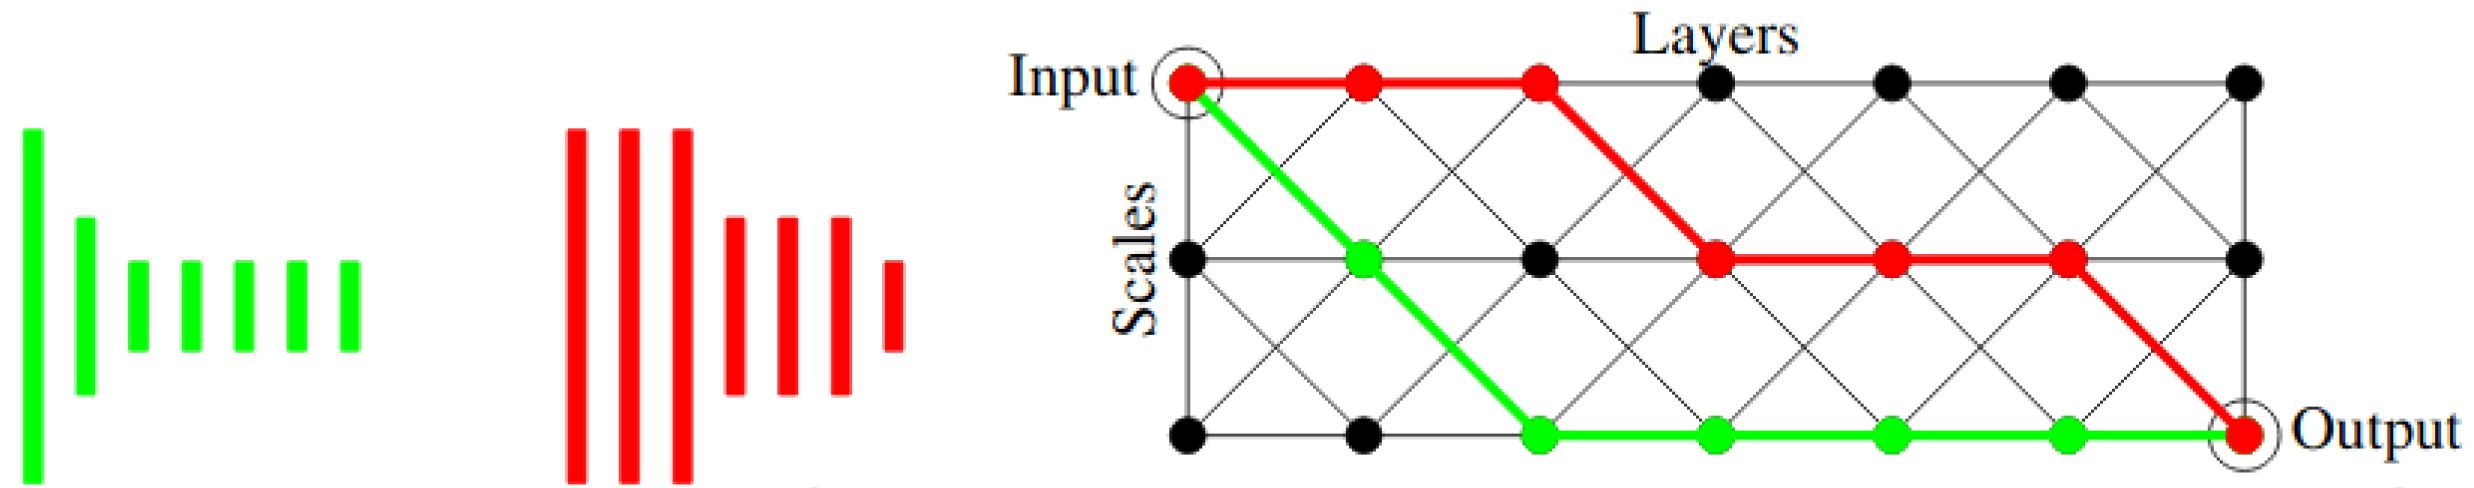
\includegraphics[width=0.7\textwidth]{images/conv_fabric_1.png}\\}
	\only<6>{\hspace*{-0.91cm}\vspace*{0.3cm}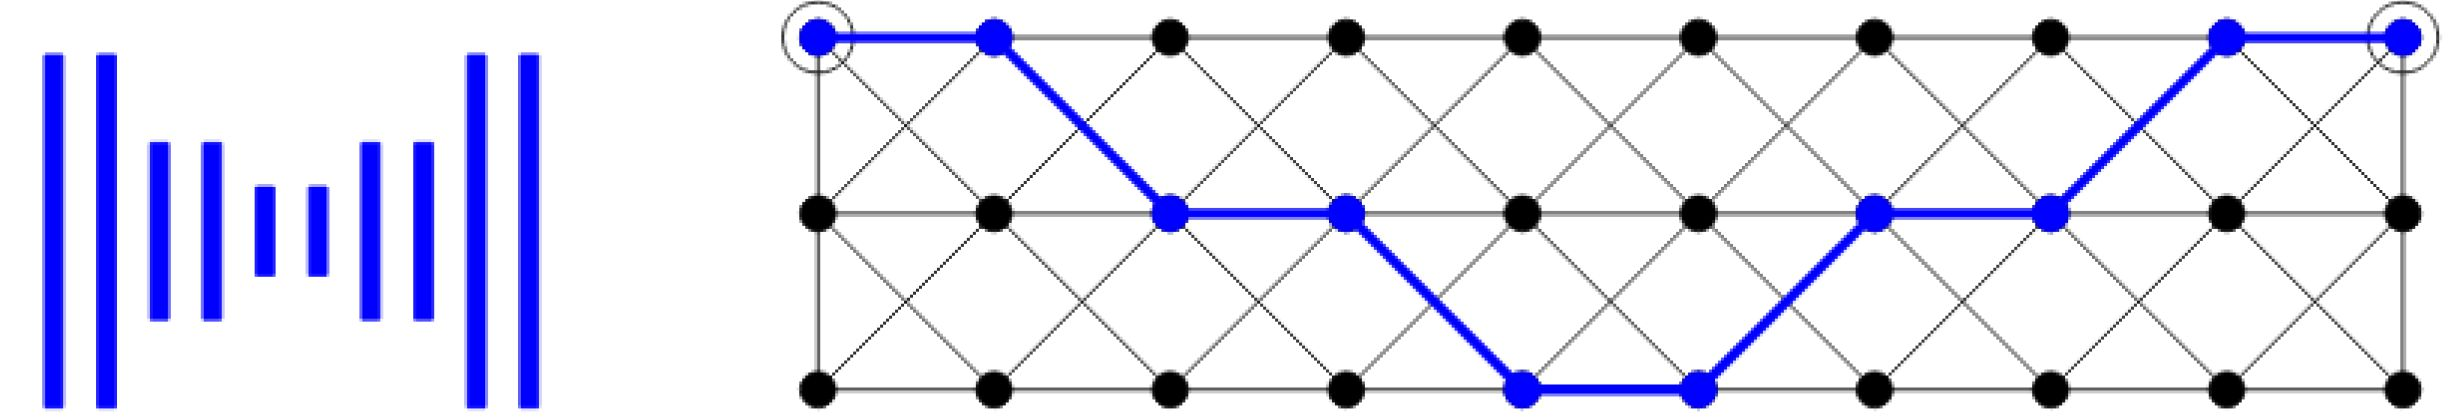
\includegraphics[width=1.02\textwidth]{images/conv_fabric_3.png}\vspace*{-0.5cm}}
	
	\only<2>{\bigskip\bigskip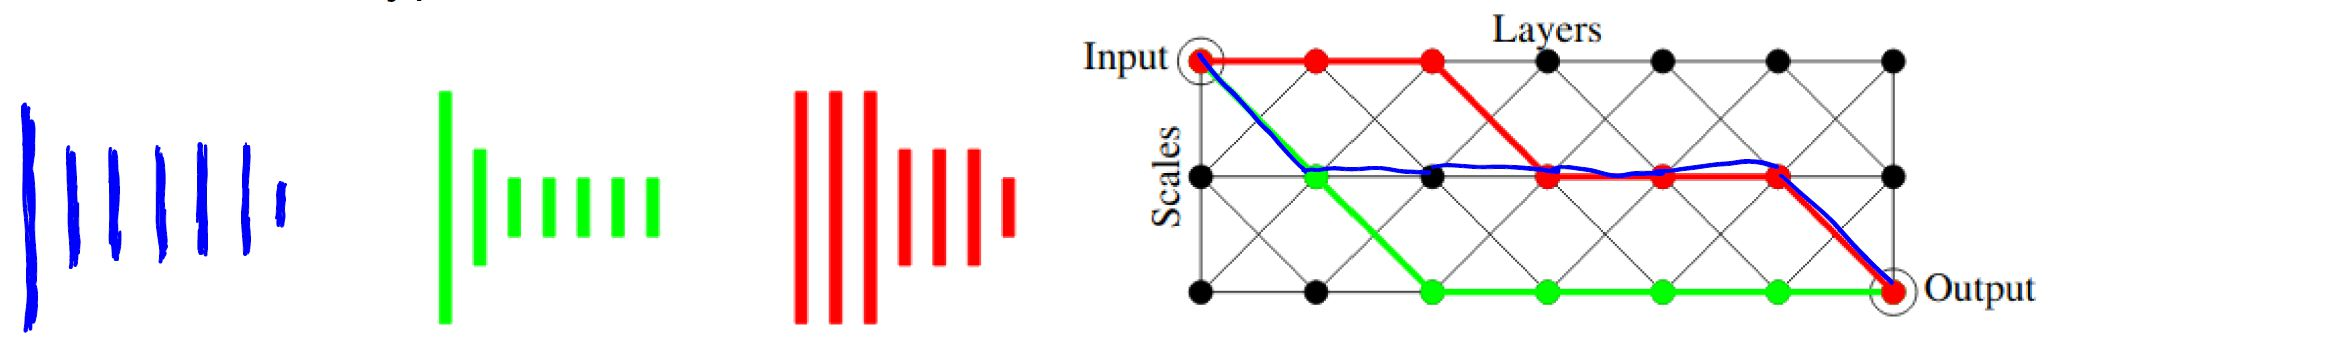
\includegraphics[width=0.7\textwidth]{images/conv_fabric_2.png}}
\pause
	\medskip
		\myit{
			\item \alert{Each path} from the input to the output \alert{represents an architecture}
	\pause
	\smallskip
			\item The \alert{nodes represent tensors}
			\item The \alert{edges represent computations} (e.g., convolution / strided convolution)
	\pause
	\smallskip
		\item \alert{Weights for the operation on an edge are shared}\\ across all (exponentially many) architectures that have that edge
		}
	}
%\pause
%\bigskip
%	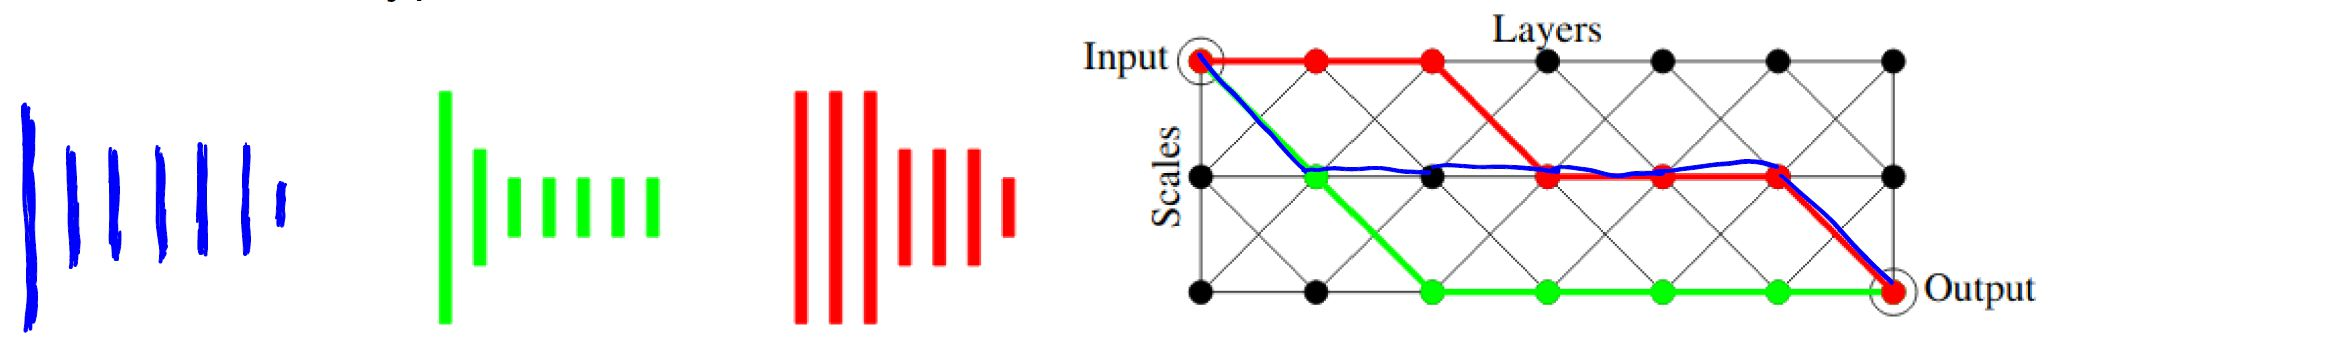
\includegraphics[width=0.7\textwidth]{images/conv_fabric_2.png}
	
}
%----------------------------------------------------------------------

%-----------------------------------------------------------------------
\myframetop{One-shot models for cell search spaces}{

\vspace*{-0.2cm}
\myit{
	\item \alert{Directed acyclic multigraph} to capture all (exponentially many) cell architectures		
		\myit{
			\item The \alert{nodes represent tensors}
			\item The \alert{edges represent computations} (e.g., 3x3 conv, 5x5 conv, max pool, \ldots)
			\item The results of operations on multiple edges between two nodes are combined (addition/concatenation) 
		}
\bigskip
\visible<2->{
	\item Individual architectures are subgraphs of this multigraph
	\myit{
		\item \alert{Weights for the operation on an edge are shared}\\ across all (exponentially many) architectures that have that edge
	}		
}
%	\item This one-shot model is \alert{trained as a standard neural network} with mini-batches and stochastic optimizers.
%	\visible<2->{\item At each mini-batch iteration \alert{weights are shared} between different architectures with common edges/nodes in the supergraph}
	}
\medskip	
	\centering
	\visible<1->{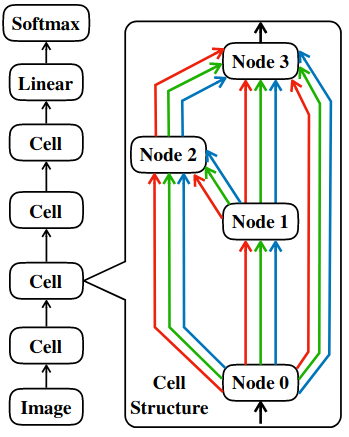
\includegraphics[width=0.19\textwidth]{images/one_shot_model_1.png}\quad\quad\quad\quad\quad\quad}
	\visible<2->{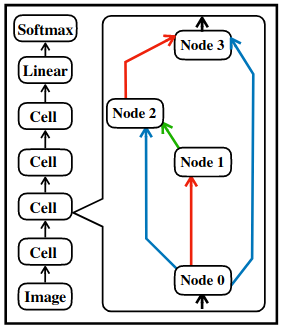
\includegraphics[width=0.19\textwidth]{images/one_shot_model_2.png}\quad\quad}
	\visible<2->{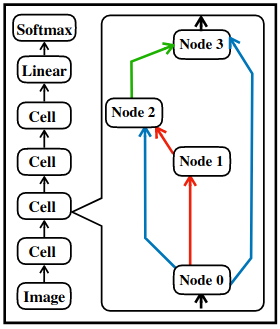
\includegraphics[width=0.19\textwidth]{images/one_shot_model_3.png}}

}
%----------------------------------------------------------------------

%-----------------------------------------------------------------------
%\myframetop{Basic Principle}{
%	\centering
%	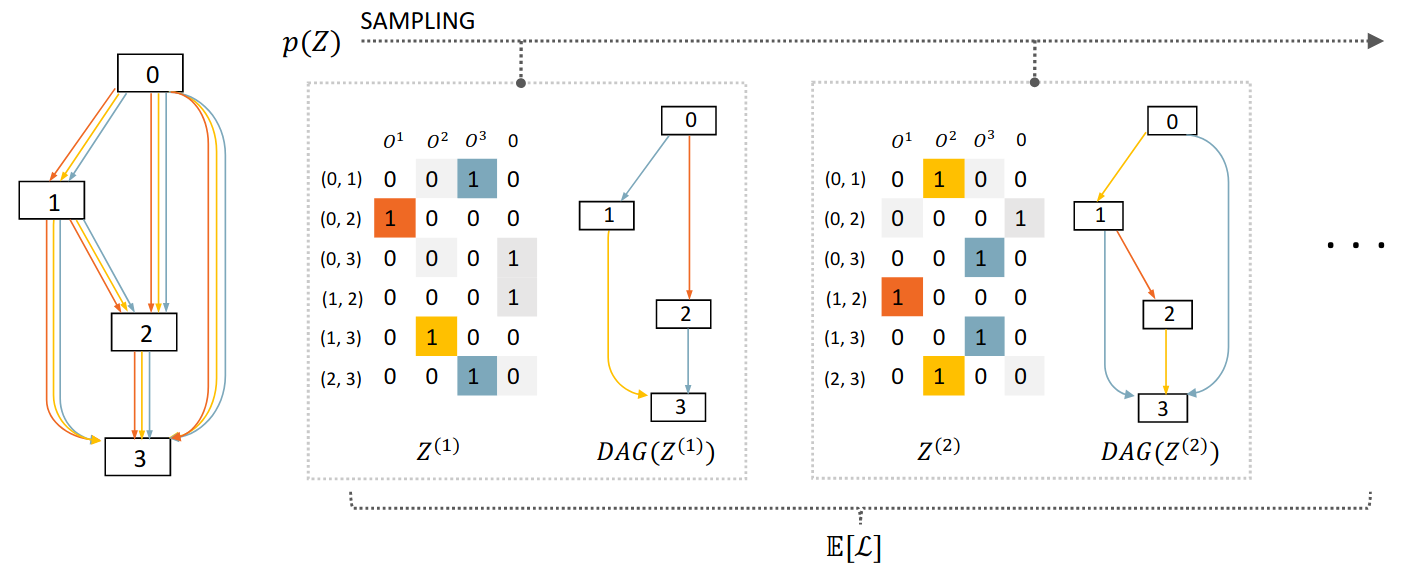
\includegraphics[width=0.7\textwidth]{images/snas_oneshot.png}
%	
%	\only<1>{
%	\begin{itemize}
%	\footnotesize
%		\item The \textbf{one-shot model} is a multi-graph containing all possible DAGs
%		\myit{
%		\footnotesize
%			\item[-] Every DAG represents a single architecture $Z^{(\cdot)}$ in the search space $\mathcal{A}$.
%			\item[-] Nodes represent aggregating operations (e.g. summation, concatenation) for incoming tensors.
%			\item[-] Edges represent operations $O^i$ (in the figure: one color per operation)
%			}
%		\item The row labels in the matrix above represent a pair of nodes $(j,k)$ in the graph and the column labels the operations $O^i$. A value of $1$ means that that operaration is active in the edge connecting node $j$ to $k$.
%	\end{itemize}
%	}
%
%	\only<2>{
%	\begin{itemize}
%	\footnotesize
%		\item The most important principle in one-shot models is \textbf{weight-sharing} between graphs.
%		\myit{
%		\footnotesize
%			\item[-] The one-shot model is trained as a normal neural network, i.e. with mini-batch training. The question is how to distinguish single architectures in the one-shot model during this training?
%			\item[-] One way is that for each sampled mini-batch also sample stochastically an architecture (DAG) and update only the parameters of that architecture.
%			\item[-] For all subsequent iterations in case a new sampled architecture has common edges (i.e. some entries in the matrices are the same) in the DAG, the weights are shared.
%			}
%	\end{itemize}
%	}
%}
%----------------------------------------------------------------------


\myframetop{Training the one-shot model -- standard SGD \litw{\href{https://arxiv.org/pdf/1606.02492.pdf}{Saxena and Verbeek. 2017}}}{

	\myit{
\visible<1->{
		\item One-shot model is an acyclic graph; thus, backpropagation applies
		\myit{
			\item Simplest method: standard training with SGD
			\item This implicitly trains \alert{an exponential number of architectures}
%			\item Used by convolutional neural fabrics		
		}
}
\medskip

%		\myit{
%			\item They did not aim at extracting a strong single architecure
%			\item Rather, they aimed for a good ensemble
%		}
%\pause
%\medskip
\visible<2->{
		\item Potential issue: co-adaptation of weights
		\myit{
			\item Weights are implicitly optimized to work well on average across all architectures
			\item They are \alert{not} optimized specifically for the top-performing architecture
		}
}
	}
\bigskip
	\centering
	\visible<1->{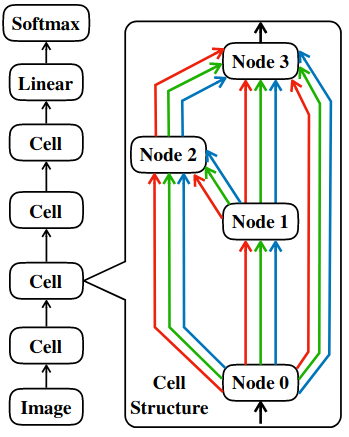
\includegraphics[width=0.2\textwidth]{images/one_shot_model_1.png}}
}
%----------------------------------------------------------------------

%----------------------------------------------------------------------

%\myframetop{Impact of DropPath \litw{\href{http://proceedings.mlr.press/v80/bender18a/bender18a.pdf}{Bender et al., 2018}}}{
%	\centering
%	
%	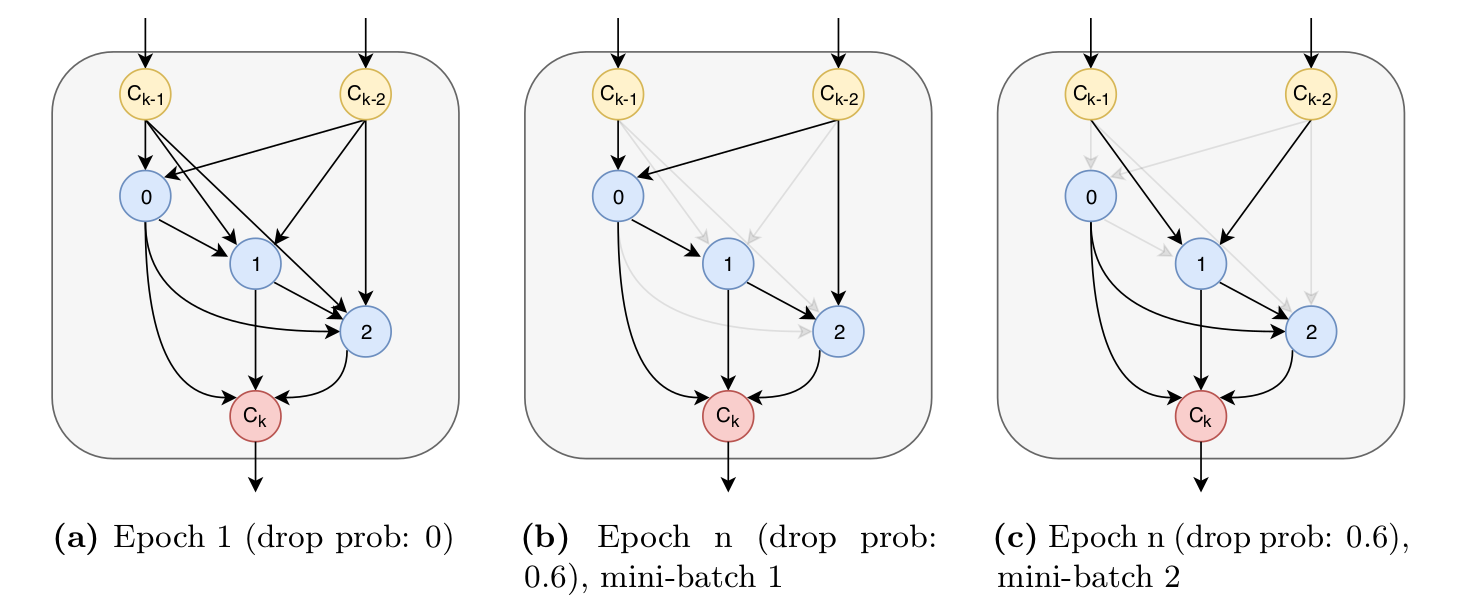
\includegraphics[width=0.8\textwidth]{images/droppath.png}
%	
%    \begin{itemize}
%		\item DropPath zeros out one a subset of the operations at each mini-batch training iteration with probability $p$.
%		\item ScheduledDropPath starts with $p=0$ and increases that linearly throughout training until a maximum $p_{max}$ in the end.
%	\end{itemize}
%}
%---------------------------------------------------------------



%----------------------------------------------------------------------
\myframetop{Training the one-shot model -- DropPath \litw{\href{http://proceedings.mlr.press/v80/bender18a/bender18a.pdf}{Bender et al. 2018}}}{
	\centering
	
	\begin{itemize}
	%\footnotesize
		\item To avoid coadaptation of weights, we can use \alert{DropPath}, a technique analogous to Dropout \lit{\href{http://jmlr.org/papers/v15/srivastava14a.html}{Srivastava et al., 2014}}:
		\myit{
\visible<2->{
			\item[-] At each mini-batch iteration:\\ for each operation connecting 2 nodes, zero it out with probability $p$
}
\smallskip
\visible<3->{
			\item[-] \alert{ScheduledDropPath}: starts with $p=0$ and increases $p$ linearly to $p_{max}$ at the end of training
}
			}
	\end{itemize}
	
\vspace*{-0.5cm}
\begin{columns}
	\column{0.01\textwidth}
	\column{0.33\textwidth}
	
	\begin{center}
	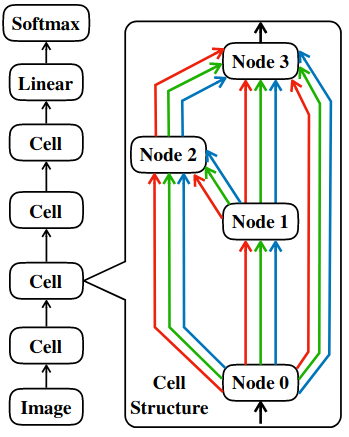
\includegraphics[width=0.6\textwidth]{images/one_shot_model_1.png}\\
	One-shot model
	\end{center}
	
	\column{0.02\textwidth}
	\column{0.33\textwidth}	
	\begin{center}
\visible<2->{	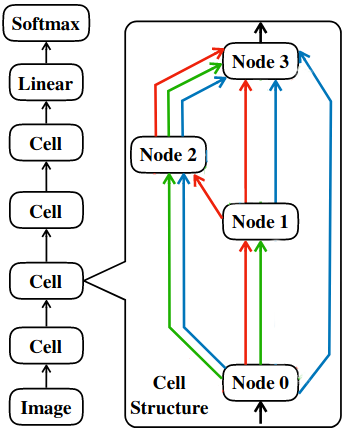
\includegraphics[width=0.6\textwidth]{images/drop_path_1.png}\\
	Architecture for batch 1
}
	\end{center}
	
	\column{0.33\textwidth}	
	\begin{center}
\visible<2->{
	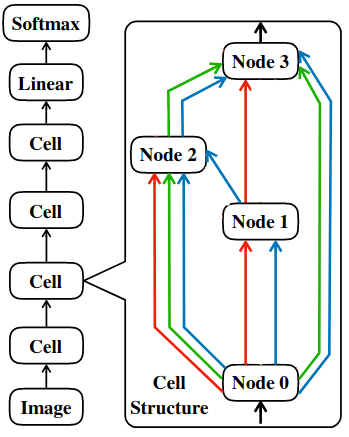
\includegraphics[width=0.6\textwidth]{images/drop_path_2.png}\\
	Architecture for batch 2
}
	\end{center}	

	\column{0.02\textwidth}	
\end{columns}
%	
%	\only<1->{
%	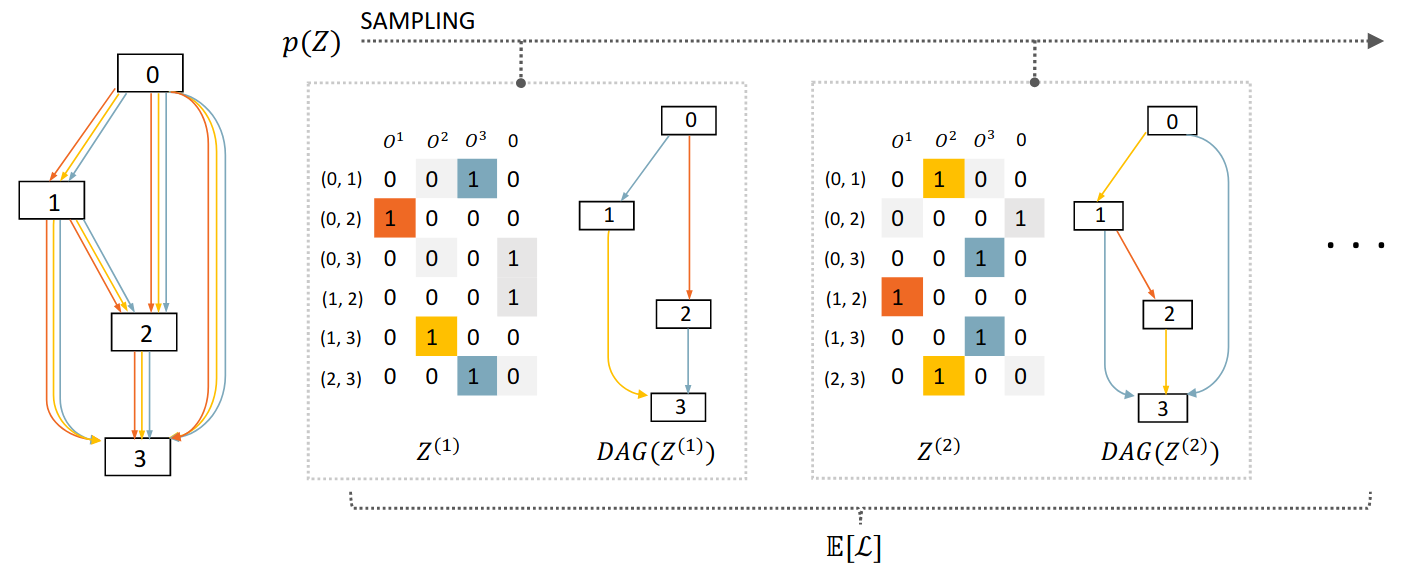
\includegraphics[width=.75\textwidth]{images/snas_oneshot.png}
%	}
}
%---------------------------------------------------------------


%----------------------------------------------------------------------
\myframetop{Training the one-shot model -- Sampling}{
	\centering
	
    \begin{itemize}
		\item At each mini-batch iteration during the training of the one-shot model \alert{sample a single architecture} 
		%$Z$ 
		from the search space 
		%$\mathcal{A}$.
		\visible<3->{
		\myit{
			\item[-] \textbf{Random Search with Weight Sharing} \lit{\href{https://arxiv.org/pdf/1902.07638.pdf}{Li and Talwalkar. 2020}} $\longrightarrow$ sample from uniform distribution
			\item[-] \textbf{ENAS} \lit{\href{https://arxiv.org/pdf/1802.03268.pdf}{Pham et al. 2018}} $\longrightarrow$ sample from the learned policy of a RNN controller
		}
		}
\pause
\medskip
		\item \alert{Update the parameters of the one-shot model} corresponding to only that architecture
	\end{itemize}
	
\vspace*{-0.5cm}
\begin{columns}
	\column{0.01\textwidth}
	\column{0.33\textwidth}
	
	\begin{center}
	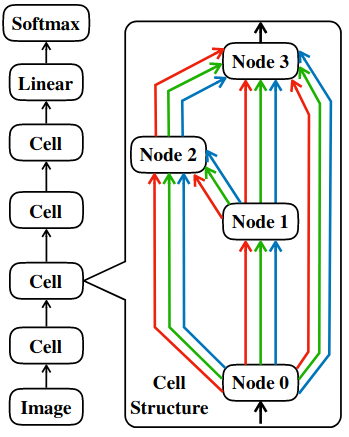
\includegraphics[width=0.6\textwidth]{images/one_shot_model_1.png}\\
	One-shot model
	\end{center}
	
	\column{0.02\textwidth}
	\column{0.33\textwidth}	
	\begin{center}
	\smallskip
	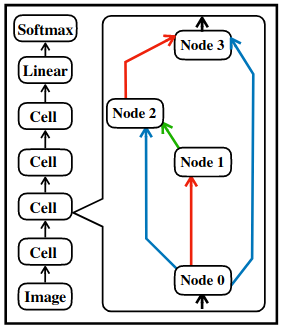
\includegraphics[width=0.6\textwidth]{images/one_shot_model_2.png}\\
	Architecture for batch 1
	\end{center}
	
	\column{0.33\textwidth}	
	\begin{center}
	\smallskip
	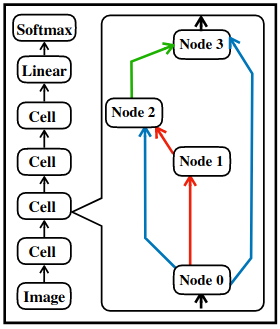
\includegraphics[width=0.6\textwidth]{images/one_shot_model_3.png}\\
	Architecture for batch 2
	\end{center}	

	\column{0.02\textwidth}	
\end{columns}
%	
%	\only<1->{
%	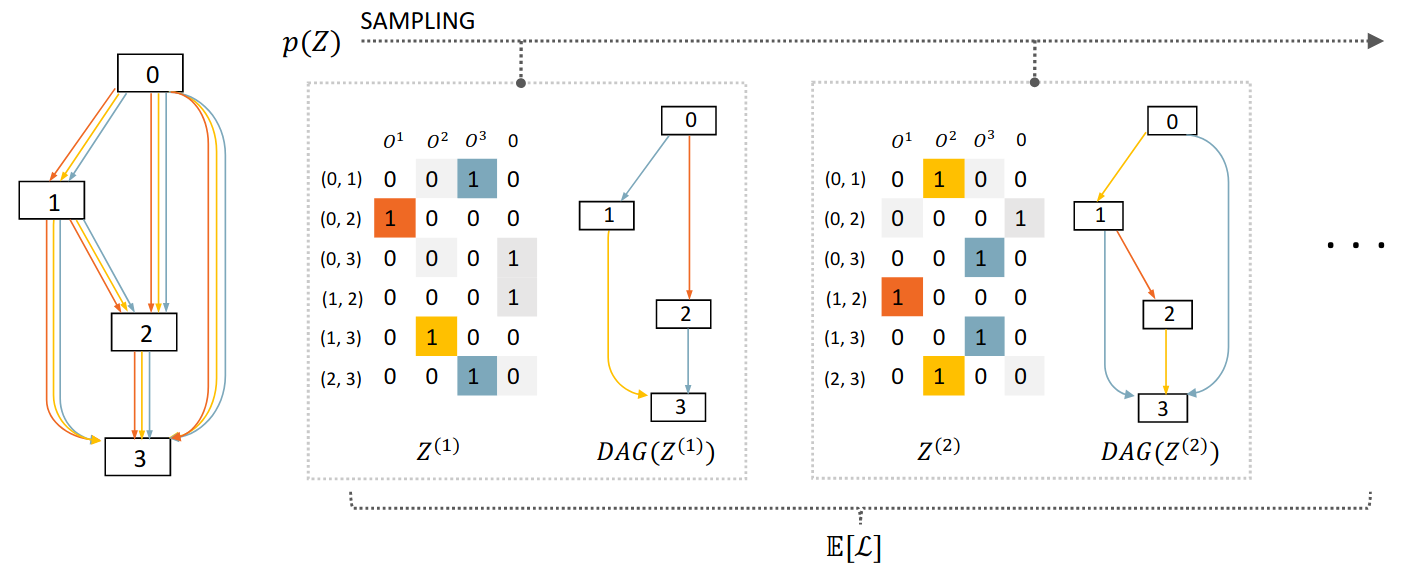
\includegraphics[width=.75\textwidth]{images/snas_oneshot.png}
%	}
}
%---------------------------------------------------------------


%----------------------------------------------------------------------

%\myframetop{Random Search with Weight Sharing \litw{\href{https://arxiv.org/pdf/1902.07638.pdf}{Li and Talwalkar, 2020}}}{
%	\centering
	
%    \begin{itemize}
%		\item Random Search with Weight Sharing \textbf{utilizes the one-shot model to speed up vanilla random search} as follows:
%		\myit{
%			\only<1>{
%			\item[-] At each mini-batch iteration during the training of the one-shot model \alert{sample uniformly at random} one architecture $Z$ from the search space $\mathcal{A}$.
%			\item[-] \alert{Update the parameters of the one-shot model} corresponding to only that architecture.
%			\item[-] After training the one-shot model finishes, sample uniformly at random $M$ architectures and rank them based on the error on a single mini-batch from the validation set \alert{using the one-shot model parameters} (retraining from scratch is computationaly expensive).
%			\item[-] Select the top $K$, where $K < M$, and evaluate those on the full validation set, again using the one-shot parameters.
%			\item[-] Return the top performing architecture to \alert{retrain from scratch}.
%			}
%			\only<2>{
%			\item[-] Works \alert{comparably to state-of-the-art NAS methods} on many benchmarks.
%			}
%		}
%	\end{itemize}
%	
%	\only<2>{
%	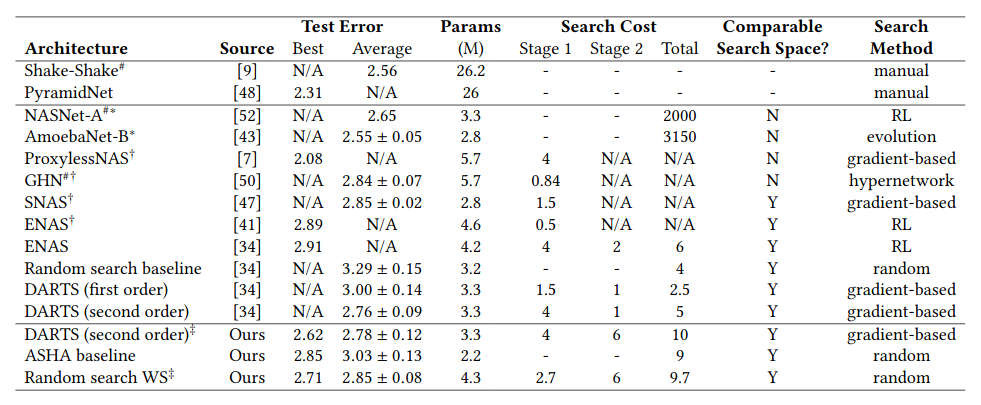
\includegraphics[width=.75\textwidth]{images/rs_ws.png}
%	}
%}
%---------------------------------------------------------------

\myframetop{How to utilize the trained one-shot model?}{
	\centering
	
    \begin{itemize}
		\item After training the one-shot model we have to \alert{select the best individual architecture} from it
		\item There are multiple ways one can approach this. Some of these are:
		\myit{
\pause
			\item[$1$.] Sample uniformly at random $M$ architectures and rank them based on their validation error \alert{using the one-shot model parameters} 
			%(retraining from scratch is computationaly expensive)
			%\item[-] Select the top $K$, where $K < M$, and evaluate those on the full validation set, again using the one-shot parameters.
\pause
			\item[$1b$.] (Optional) Select top $K$ ($K<M$) and retrain them from scratch for a couple of epochs
\pause
			\item[$2$.] Return the top performing architecture to \alert{retrain from scratch} for longer
		}
	\end{itemize}
	
	\onslide<5>{
    	\begin{minipage}{0.4\textwidth}
        	\begin{itemize}
				\footnotesize
				\item \textbf{Pitfall:} the correlation between architectures evaluated with the one-shot weights and retrained from scratch (stand-alone models) should be high
				\item If not, \textbf{selecting the best architecture based on the one-shot weights} is sub-optimal.
			\end{itemize}
	    \end{minipage}
	    \hspace{1cm}
    	\begin{minipage}{0.5\textwidth}
\begin{center}
	        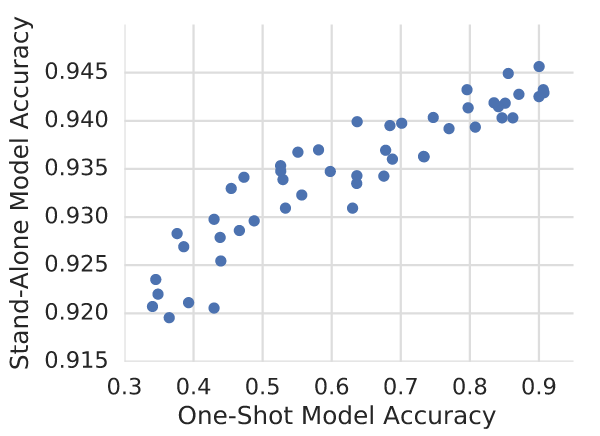
\includegraphics[width=.7\textwidth]{images/bender_correlation_1.png}\\
	        \scriptsize{From \smaller{\lit{\href{http://proceedings.mlr.press/v80/bender18a/bender18a.pdf}{Bender et al. 2018}}}}
\end{center}
    	\end{minipage}
	}
}
%---------------------------------------------------------------

%----------------------------------------------------------------------
\myframe{Questions to Answer for Yourself / Discuss with Friends}{

	\myit{
		\item Repetition:\\ \alert{How are the weights shared in the one-shot model?}
\bigskip
		\item Repetition:\\ \alert{What is the difference between Random Search with Weight Sharing and ENAS?}
\medskip
		\item Discussion:\\ \alert{What migth be some downsides of using the one-shot model for NAS?}
	}	 
}
%-----------------------------------------------------------------------

